\section{Capabilities (Architectural Framework)}
\label{sec:arch}


\begin{figure*}[!t]
		\centering
		\resizebox{\textwidth}{!}{%
		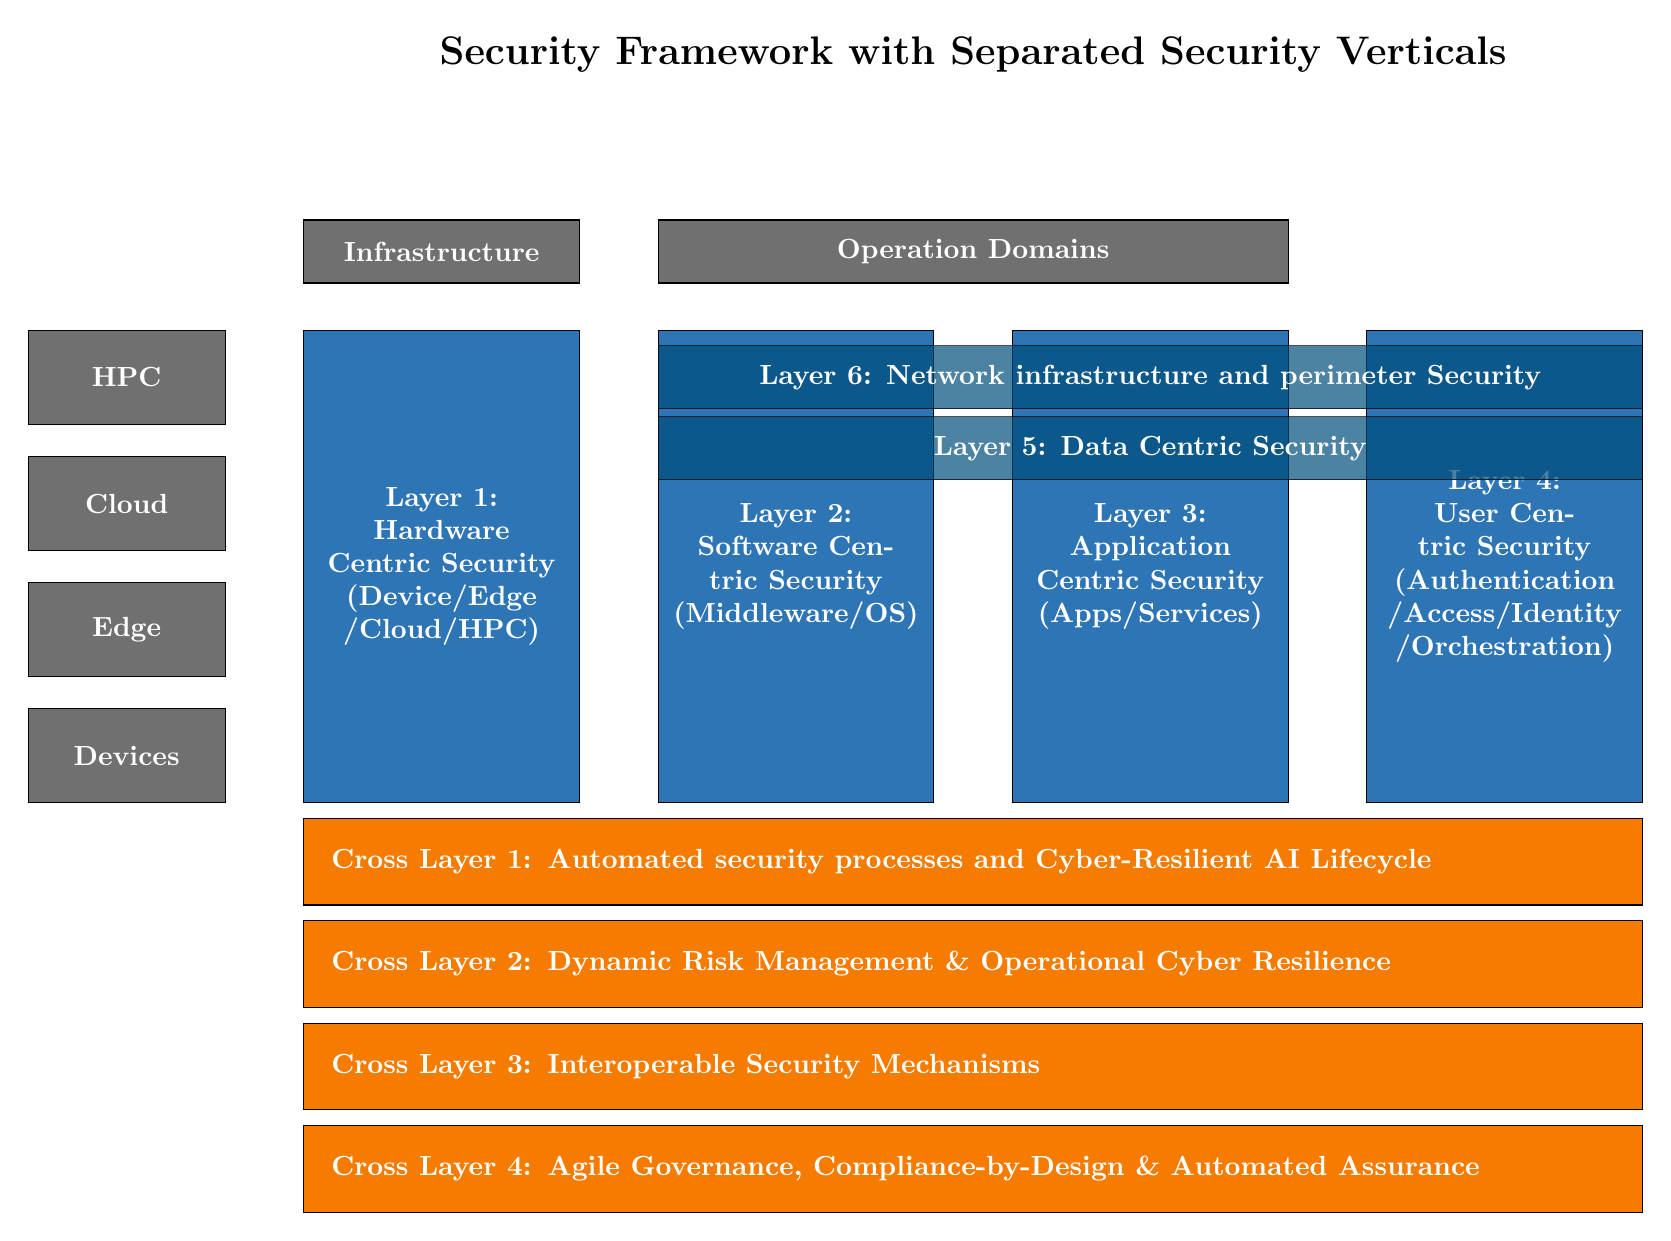
\begin{tikzpicture}[every node/.style={font=\small}]
			% Define colors
			\definecolor{archblue}{RGB}{46, 117, 182}
			\definecolor{sec_verticals_bg}{RGB}{245, 124, 0}
			\definecolor{env_bg}{RGB}{112, 112, 112}
			\definecolor{overlay}{RGB}{0, 77, 122}

			% Styles
			\tikzstyle{arch_col} = [fill=archblue, draw=black, text=white, font=\bfseries, minimum width=3.5cm, minimum height=6cm, align=center, text width=3.2cm]
			\tikzstyle{env_box} = [fill=env_bg, draw=black, text=white, font=\bfseries, minimum width=2.5cm, minimum height=1.2cm, align=center]
			\tikzstyle{top_tool} = [draw=black, fill=env_bg, text=white, minimum height=0.8cm, align=center, font=\bfseries]
			\tikzstyle{overlay_box} = [fill=overlay, draw=black, text=white, font=\bfseries, minimum height=0.8cm, align=center, opacity=0.7, text opacity=1]
			\tikzstyle{vertical_box} = [fill=sec_verticals_bg, draw=black, text=white, font=\bfseries, minimum width=17.0cm, minimum height=1.1cm, align=left, text width=16.3cm]

			% Column X positions
			\def\colone{-4.5}
			\def\coltwo{0}
			\def\colthree{4.5}
			\def\colfour{9}
            \pgfmathsetmacro{\layerSpanLeft}{\coltwo-1.75}
            \pgfmathsetmacro{\layerSpanRight}{\colfour+1.75}
            \pgfmathsetmacro{\layerSpanCenter}{(\layerSpanLeft+\layerSpanRight)/2}
            \pgfmathsetmacro{\layerSpanWidth}{\layerSpanRight-\layerSpanLeft}

			% Environment boxes (left)
			\node[env_box] at (-8.5, 2.4) {HPC};
			\node[env_box] at (-8.5, 0.8) {Cloud};
			\node[env_box] at (-8.5, -0.8) {Edge};
			\node[env_box] at (-8.5, -2.4) {Devices};

			% Main architecture columns representing layers
			\node[arch_col] (hw) at (\colone, 0) {Layer 1: \\ Hardware Centric Security \\ (Device/Edge\\ /Cloud/HPC)};
			\node[arch_col] (mw) at (\coltwo, 0) {Layer 2: \\ Software Centric Security \\ (Middleware/OS)};
			\node[arch_col] (app) at (\colthree, 0) {Layer 3: \\ Application Centric Security \\ (Apps/Services)};
			\node[arch_col] (user) at (\colfour, 0) {Layer 4: \\ User Centric Security \\ (Authentication\\ /Access/Identity\\ /Orchestration)};

			% Top tooling boxes
			\node[top_tool, minimum width=3.5cm] at (\colone, 4) {Infrastructure};
			\node[top_tool, minimum width=8cm] at (2.25, 4) {Operation Domains};

			% Arrows from tooling
			\draw[->, line width=2pt, white] (\colone, 3.5) -- (\colone, 3.1);
			\draw[->, line width=2pt, white] (2.25, 3.5) -- (2.25, 3.1);

			% Other layers as overlays/headers
			\node[overlay_box, minimum width=12.5cm] at (4.5, 1.5) {Layer 5: Data Centric Security};
            \node[overlay_box, minimum width=\layerSpanWidth cm] at (\layerSpanCenter, 2.4) {Layer 6: Network infrastructure and perimeter Security};

			% Separated vertical boxes
			\node[vertical_box] at (2.25, -3.75) {\textbf{Cross Layer 1: Automated security processes and Cyber-Resilient AI Lifecycle}};
			\node[vertical_box] at (2.25, -5.05) {\textbf{Cross Layer 2: Dynamic Risk Management \& Operational Cyber Resilience}};
			\node[vertical_box] at (2.25, -6.35) {\textbf{Cross Layer 3: Interoperable Security Mechanisms}};
			\node[vertical_box] at (2.25, -7.65) {\textbf{Cross Layer 4: Agile Governance, Compliance-by-Design \& Automated Assurance}};

			% Title
			\node[font=\Large\bfseries, anchor=center] at (2.25, 6.5) {Security Framework with Separated Security Verticals};

		\end{tikzpicture}%
		}
		\caption{Security Framework with separated security verticals in dedicated boxes.}
		\label{fig:security_framework_verticals_boxes}
    \end{figure*}

As it is illustrated in Figure~\ref{fig:security_framework_verticals_boxes}, the roadmap is structured across a cohesive architectural framework that spans four continuum environments (HPC, Cloud, Edge, Devices). The capabilities are organized into Six Security Layers (The Vertical Stack) and Four Transversal Cross-Layers (The Horizontal Enablers).

\subsection*{Part A: The Security Layers (Vertical Stack)}
These layers define the specific technical security controls implemented across the computing infrastructure.

\subsubsection*{Layer 1: Hardware-Centric Security}
\textbf{1.1 Hardware Roots of Trust:} Cryptographically verifiable supply chain trust (e.g., TPM attestation, secure enclaves) ensures physical device integrity. Success depends on driving European open-hardware designs (e.g., RISC-V) toward \textbf{EUCC 'High' assurance level certification} \cite{eucc} to mathematically guarantee resistance against state-level physical tampering and side-channel attacks at the vulnerable far-edge.
\textbf{1.2 Physical-Layer (PHY) Threat Detection \& Fingerprinting:} Exploiting intrinsic wireless channel characteristics, such as Channel State Information (CSI), Carrier Frequency Offset (CFO), and Received Signal Strength Indicator (RSSI). That is to establish real-time, keyless device authentication and anomaly detection at the lowest layer of the stack. This provides a hardware-anchored security primitive that is resilient even when upper-layer cryptographic processing is compromised or infeasible.

\subsubsection*{Layer 2: Software-Centric Security (Mid\-dle\-ware/OS)}

\textbf{2.1 OS \& Middleware Hardening:} Securing hypervisors, container runtimes, and distributed operating systems is critical for isolation. This involves hardening KVM/QEMU and supporting sovereign, lightweight Linux distributions optimized for edge resource constraints, ensuring a reduced attack surface for the cognitive continuum.

\textbf{2.2 Secure OTA Patch \& Update Management:} Edge nodes deployed in the field---smart grids, O-RAN radios, industrial gateways---require cryptographically verified, failure-resilient over-the-air (OTA) update pipelines. A compromised or failed update mechanism can render entire fleets of field-deployed nodes permanently vulnerable, making robust OTA management a critical software-layer capability.

\subsubsection*{Layer 3: Application-Centric Security (Apps/Services)}

\textbf{3.1 Workload Security:} Securing containerized applications, microservices, and serverless functions executing dynamically across multi-provider nodes. This is achieved through hardened service meshes and sidecar proxy architectures that provide mutual TLS and granular traffic inspection without impacting performance.

\textbf{3.2 In-Band Network Telemetry (INT) \& Deep Observability:} Embedding ``smart telemetry'' directly into the data packets traversing containerized workloads and service meshes, providing granular, real-time visibility into network behaviour and performance without requiring out-of-band monitoring infrastructure. This feeds high-fidelity signals to security analytics platforms.

\textbf{3.3 API Security Gateway \& Policy Enforcement:} As containerized AI workloads increasingly communicate through REST/gRPC APIs, a dedicated API security gateway provides a unified enforcement point for authentication tokens, rate limiting, schema validation, and payload inspection---preventing injection attacks and data exfiltration at the application boundary.


\subsubsection*{Layer 4: User \& Orchestration-Centric Security}
\textbf{4.1 Zero-Trust Orchestration:} Seamless policy enforcement across a multi-provider computing continuum requires robust Policy Enforcement Point (PEP) and Policy Decision Point (PDP) architectures. This enables continuous authorization and dynamic access controls that adapt to the context of the request.

\textbf{4.2 Federated Identity \& Access Management (IAM):} Cross-domain identity federation and verifiable credentials for machines, users, and automated workloads. Implementing \textbf{Self-Sovereign Identity (SSI)} principles allows for cryptographically secure, decentralized authentication across heterogeneous cloud-edge domains.

\textbf{4.3 Privileged Access Management (PAM) \& Just-In-Time (JIT) Access:} Lateral movement by attackers frequently exploits over-provisioned standing privileges---the precise vector behind major Advanced Persistent Threat (APT) campaigns. PAM and JIT access controls ensure that elevated privileges are granted only for defined, time-bounded sessions with full auditability, minimizing the blast radius of any credential compromise.

\subsubsection*{Layer 5: Data-Centric Security}
\textbf{5.1 End-to-end Confidential Computing:} Data-in-use security through Trusted Execution Environments (TEEs) spanning the entire Cloud-to-IoT data path. Leveraging TEE abstraction layers and remote attestation ensures that sensitive European data remains encrypted even during processing in non-trusted environments.

\textbf{5.2 Post-Quantum \& Cryptographic Agility:} PQC standardization and hybrid crypto deployment are necessary to secure long-lived data. Priority is placed on \textbf{PQC migration for resource-constrained devices}, ensuring that edge infrastructure is resilient against ``Harvest Now, Decrypt Later'' quantum threats.

\textbf{5.3 Signaling (Data) Security:} Moving beyond best-effort packet forwarding by embedding trust directly into the network signaling architecture. This ensures the integrity and authenticity of control-plane messages, preventing hijacking of routing decisions and network configuration across the distributed continuum.

\textbf{5.4 Distributed Reputation \& Trust Networking:} Implementing a ubiquitous, real-time reputation system built on Distributed Ledger Technology (DLT) and smart contracts. This enables autonomous, evidence-based trust decisions about nodes, services, and data sources across the continuum without reliance on a central authority.

\textbf{5.5 Quantum Key Distribution (QKD) for Critical Links:} While PQC addresses algorithmic quantum-resistance, QKD provides information-theoretically secure key exchange over optical fibre for point-to-point high-value links (government, critical infrastructure backbone). These two technologies are complementary and together form a comprehensive quantum-safe strategy.

\textbf{5.6 Secure Multi-Party Computation (SMPC):} Homomorphic Encryption and TEEs (Layer 5.1) handle confidential computing for single-party workloads. SMPC enables multiple mutually distrusting parties to jointly compute a function over their combined private inputs without revealing those inputs to each other---a critical capability for cross-border analytics and federated AI in regulated sectors.

\subsubsection*{Layer 6: Network Infrastructure \& Perimeter-Centric Security}
\textbf{6.1 Telco-cloud \& O-RAN Security:} Hardening distributed 5G/6G cores and RAN components must align with the \textbf{Smart Networks and Services Joint Undertaking (SNS JU) SRIA} \cite{snsju}. This ensures sovereign control over network slice isolation and virtualized RAN components.

\textbf{6.2 Cross-Sector Physical Resilience \& Safety:} Adapting strict network controls and IT/OT gateway security for high-availability edge environments (e.g., Smart Grids). This guarantees that cyber-breaches in the digital layer do not cascade into physical safety hazards or kinetic damage in critical infrastructure.

\textbf{6.3 Edge-Native Autonomous Guardians:} Hosting lightweight, localized security control functions (Security-as-a-Service aggregators) directly at the far-edge gateways or within Open-RAN Radio Intelligent Controllers (RIC). These autonomous guardian nodes execute real-time threat mitigation without requiring round-trip communication to a centralized cloud-based SOC, dramatically reducing response latency.

\textbf{6.4 Non-Terrestrial Network (NTN) \& Satellite Security:} 6G will natively integrate satellite segments for coverage continuity, backhaul resilience, and emergency operations. These non-terrestrial links introduce distinct threat surfaces---including signal interception and orbital spoofing---requiring dedicated security requirements aligned with 3GPP NTN specifications and the EU Space Programme.

\subsection*{Part B: The Transversal Security Verticals (Cross-Layers)}
These four cross-layers represent continuous, automated processes and governance structures that intersect every layer of the vertical stack.

\subsubsection*{Cross-Layer 1: Automated Security Processes \& Cyber-Resilient AI Lifecycle}
\textbf{CL1.1 Continuous DevSecOps (Shift-Left):} Embedding AI-driven code analysis and automated vulnerability remediation at the earliest stages of the software lifecycle.

\textbf{CL1.2 Model \& Pipeline Integrity (DataBOMs):} Securing AI training pipelines to prevent data poisoning and unauthorized model manipulation.

\textbf{CL1.3 Runtime AI Defense:} Defending AI/ML infrastructure against real-world adversarial attacks (e.g., prompt injection, model evasion/theft) at the edge.

\textbf{CL1.4 Dynamic Supply Chain Verification (Runtime SBOMs):} Moving beyond static software manifests by implementing dynamic Software Bill of Materials (Runtime SBOMs) and ``cryptographic proof of execution'' to continuously verify the integrity of containerized microservices and AI components as they migrate across the multi-provider edge-cloud continuum.

\textbf{CL1.5 Automated Adversarial Testing \& Continuous Purple Teaming:} DevSecOps pipelines focus on code analysis and remediation; the adversarial counterpart provides continuous automated penetration testing, fuzzing (coverage-guided and protocol-level), and purple-team automation that simulates real attacker behaviour against live staging environments, ensuring defenses are validated continuously rather than at periodic intervals.


\subsubsection*{Cross-Layer 2: Dynamic Risk Management \& Operational Cyber Resilience}
\textbf{CL2.1 Automated SOC Operations \& Collaborative Threat Intelligence:} Continuous monitoring, SOC federation across Member States, and automated incident containment, underpinned by legally protected, cross-border threat intelligence sharing ecosystems designed to overcome institutional trust barriers and incentivize active collaboration \cite{concordia}.

\textbf{CL2.2 Systemic \& Cascading Risk Mitigation:} Mapping the evolving threat landscape and using impact-likelihood scoring to dynamically sever links and prevent cross-domain systemic failures.

\textbf{CL2.3 High-Precision Telemetry and Security Signalling:} Implementing ``smart telemetry'' and cybersecurity-related signalling to feed real-time threat intelligence into analytics platforms without overwhelming network bandwidth---ensuring that visibility does not itself become an attack vector or performance bottleneck.

\textbf{CL2.4 Internet of Behavior (IoB) and Evidence Sharing:} Utilizing cybersecurity and QoS signalling traffic to extract and share behavioral patterns across the infrastructure, establishing an ``Internet of Behavior'' that enables proactive anomaly correlation and evidence-based risk assessment at continental scale.

\textbf{CL2.5 AI-Native Analytics Integration (NWDAF \& LLMSecOps):} Routing cybersecurity signalling traffic and telemetry through centralized analytics hubs powered by AI agents. This creates a live ``nervous system'' for the network, allowing AI agents to continuously monitor for zero-day exploits, analyze encrypted traffic flows, and trigger automated incident responses aligned with NWDAF (Network Data Analytics Function) standards.

\textbf{CL2.6 Cyber Threat Intelligence (CTI) Lifecycle Management:} While CL2.1 and CL2.4 consume and act on threat data, explicit governance of the full CTI lifecycle---collection, processing, analysis, dissemination, and feedback---is required as a prerequisite for the federated SOC vision. A sovereign EU CTI platform must define this governance layer to ensure data quality, legal compliance, and attribution reliability.

\textbf{CL2.7 Cyber Deception Technology \& Active Defense (Honeynets, Canaries):} Current detection is passive---telemetry is observed and anomalies flagged. Deception adds an active intelligence-collection dimension by deploying decoy assets (honeypots, honeynets, credential canaries, fake API endpoints) that generate high-fidelity, low-noise alerts when touched, enabling early detection of advanced intrusions and insider threats.

\subsubsection*{Cross-Layer 3: Interoperable Security Mechanisms \& Open-Source Verifiability}
\textbf{CL3.1 Heterogeneous Interoperability \& Simpl Integration:} Secure communication and data exchange across disparate systems, edge nodes, and proprietary domains. This includes mandatory alignment with and integration into the Simpl open-source smart middleware \cite{cloud_edge_roadmap} to ensure secure, federated access across Common European Data Spaces.

\textbf{CL3.2 Minimal Interoperability Mechanisms (MIMs) \& Open Verifiability:} Establishing standardized, baseline security and privacy controls to ensure trust without creating vendor lock-in. This relies heavily on embracing open-source software and open hardware architectures as fundamental prerequisites for transparency, cryptographic verifiability, and the elimination of proprietary black-box vulnerabilities \cite{cloud_edge_roadmap}.

\textbf{CL3.3 Neutral Host and Multi-Tenant Isolation:} As the ecosystem shifts toward infrastructure sharing and Neutral Host models spanning wireless, optical, and cloud domains, robust isolation between tenants is critical. Security architectures must enforce Zero-Trust edge operations across different network partitions to prevent cross-tenant data leakage and privilege escalation.

\textbf{CL3.4 Pan-European NaaS Federation and Cross-Border Edge Roaming:} Establishing standardized interfaces and harmonized Network APIs (e.g., leveraging CAMARA) to interconnect the fragmented edge clouds of different European telecom operators into a unified Network-as-a-Service (NaaS) platform---enabling a ``Schengen for Cloud/AI'' where compute workloads can roam seamlessly across borders.

\textbf{CL3.5 Semantic Security Interoperability (Common Ontologies \& Data Models):} Federated SOCs and shared threat intelligence only function if participating organisations share a common semantic understanding of security events, asset taxonomies, and risk classifications. Standardized ontologies (e.g., aligned with STIX/TAXII and MITRE ATT\&CK) are a prerequisite for meaningful cross-border correlation.

\textbf{CL3.6 Cyber Range \& Digital Twin Federation for Security Validation:} Before deploying cross-border federated security configurations into production, they must be validated in high-fidelity simulation environments. ENISA already coordinates national cyber range inventories; this cross-layer would federate them into a shared EU-wide infrastructure aligned with the Cyber Solidarity Act's testing provisions.

\subsubsection*{Cross-Layer 4: Compliance-by-Design, Agile Governance \& Automated Assurance}
\textbf{CL4.1 Policy-as-Code \& Compliance-by-Design:} Technical implementation of legal requirements (OSCAL) into machine-readable rules that pre-validate workloads.

\textbf{CL4.2 Continuous Automated Auditing \& Certification Lifecycle:} Replacing ``point-in-time''  PDF certificates with real-time, telemetry-driven certification tracking for both cloud services (EUCS) \cite{eucs} and physical ICT edge products (EUCC) \cite{eucc}. This ensures that edge nodes autonomously maintain compliance by integrating mandatory vulnerability handling and cryptographic patch verification directly into their operational lifecycle, strictly aligning with EUCC maintenance and assurance rules \cite{eucc}.

\textbf{CL4.3 Post-Quantum Readiness \& Zero-Trust Architectures (ZTA):} Moving beyond traditional perimeter-based defenses by embedding continuous, AI-driven Zero-Trust verification and micro-segmentation natively into the cloud-edge infrastructure, combined with a systematic migration roadmap to post-quantum cryptographic primitives across all layers.

\textbf{CL4.4 Continuous Automated Certification:} Replacing ``point-in-time'' PDF certificates with real-time, telemetry-driven certification tracking for both cloud services (\textbf{EUCS}) and physical ICT edge products (\textbf{EUCC}), ensuring that edge nodes autonomously maintain compliance by integrating mandatory vulnerability handling and cryptographic patch verification directly into their operational lifecycle \cite{eucc}.

\textbf{CL4.5 Multicloud Key Management as a Service (KMaaS):} When AI workloads, data flows, and context flows migrate dynamically across a multi-provider computing continuum, managing cryptographic keys and access policies becomes highly complex. KMaaS provides a provider-agnostic, sovereign key lifecycle management capability that prevents key sprawl and ensures revocation propagates consistently across heterogeneous environments.

\textbf{CL4.6 Privacy-Preserving Federated Computation:} When multiple providers work on the same infrastructure, AI training and inference may require access to datasets stored across different jurisdictions and competitive boundaries. Privacy-preserving techniques (federated learning, differential privacy, SMPC) enable collaborative computation while guaranteeing that raw data never leaves its sovereign jurisdiction.

\textbf{CL4.7 Cyber Risk Quantification \& Board-Level Reporting (CRQ):} Compliance frameworks define what controls to implement. A dedicated cross-layer translates technical security posture into financial and operational risk language for decision-makers---potentially in real-time---enabling boards to make informed, evidence-based investment and risk-acceptance decisions aligned with DORA requirements.

\textbf{CL4.8 AI Trustworthiness \& Algorithmic Accountability:} As AI systems themselves become actors within the security architecture---making autonomous containment decisions, classifying threats, orchestrating responses---the trustworthiness of those AI systems becomes a security-critical concern. This layer defines explainability, auditability, and override mechanisms for AI-driven security functions, ensuring alignment with the EU AI Act for high-risk systems.

\textbf{CL4.9 Regulatory Digital Twins:} Virtualized replicas of critical infrastructure specifically to stress-test regulatory compliance against evolving laws before applying changes to the live physical continuum.
